RHODES approach to traffic signal optimization is a hierachical one with 3 layers of detail, see figure \ref{fig:rhodes_hierarchi}. They can be rougly be summarized accordingly:

\begin{enumerate}
\item The macroscopic layer performs \textit{dynamic network loading}, which involves observing changes in the aggregated flow data of the entire network due to variations in the OD matrices. This layer supplies estimates of link flows to the middle level in rough numbers eg. vehicles per hour.
\item The mesoscopic middle layer considers sectors of the network eg. an arterial. This \textit{network flow control} layer work in the detail level of platoons and average speeds. Green time is allocated to phases to accomodate the movements of the platoons and so coordination of intersections is done at this level.
\item At the lowest level is \textit{intersection control} where vehicles are handled individually (a microscopic layer). Here the green times and phase ordering suggested by the middle layer are fine tuned.
\end{enumerate}

\begin{figure}[!ht]
\begin{center}
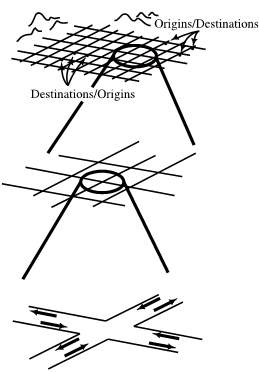
\includegraphics[scale=0.5]{rhodes_hierachy.png} 
\end{center}
\caption{The three levels of detail: network, sector, and intersection}
\label{fig:rhodes_hierarchi}
\end{figure}

An adaptive traffic control system must operate quickly in order to adapt signals to traffic in real-time. The RHODES platform has good decomposition opportunities and is pluggable ie. the upper level is a black box feeding the lower level with predictions and optimizations. At the time the article was written, the top level of RHODES had not received much development and thus only the middle and lower level are described herein.

\subsubsection*{Detection}
Detection methods are not discussed in detail in the paper. They can be of any technology including induction loops and video. 

Each link facing an intersection under intersection control are fitted with detectors to give the prediction methods optimum operating conditions. Detectors are placed in the beginning of the link so that the prediction method can use a longer horizon.

\begin{figure}[!ht]
\begin{center}
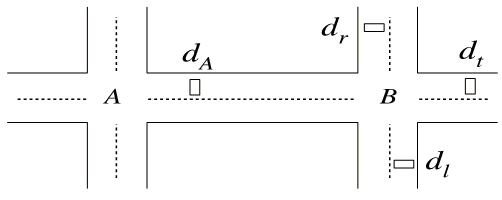
\includegraphics[scale=0.5]{rhodes_prediction-strategy.png} 
\end{center}
\caption{Detector placement and propogation of information in a simple grid}
\label{fig:rhodes_predict}
\end{figure}

\subsubsection*{Prediction}
The PREDICT method by the co-author, Head, is used to make predictions for individual vehicles. PREDICT is built for network prediction and relies on the fact that incoming flow to an intersection originates from adjacent intersections. This concept can be explained from figure \ref{fig:rhodes_predict} where traffic detected at $d_a$ is the sum of right-turning traffic at detector $d_r$, left turning traffic at $d_l$ and through-going traffic at $d_t$.

Thus given flow estimates for the links facing intersection B and turning probabilities for each link an estimate can be given for the inflow to intersection A from east. On the link between the two intersections there will be traffic entering and exiting the system, but these contributions - and losses - to the traffic, which can be measured at $d_a$, are expected to be very small.

Prediction of arrival times of the vehicles which has passed detectors $d_{\lbrace r,t,l \rbrace}$ depend on the current phase at intersection B and queue conditions. Mirchandani and Head has identified four cases, which cover arrivals to an intersection, which are summarized in table \ref{tbl:delaycases}.

\begin{table}[!ht]
\begin{center}
\begin{tabular}{l|ll}
 & \textbf{Green} & \textbf{Red} \\ \hline
\textbf{No queue} & 0 & $T_G$ \\
\textbf{Queue} & $T_Q$ & $T_G$ + $T_Q$
\end{tabular}
\end{center}
\caption{Delay incurred for a vehicle arriving to an intersection in various states where $T_Q$ is the time for ahead queue to clear and $T_G$ is the time to the next green.}
\label{tbl:delaycases}
\end{table}

In the cases involving queue there is, of course, a possibility that the vehicle will not be able to cross the intersection before several green phases have occured. This is likely to happen under high congestion when intersections are placed closely.

At the mesocopic level, network flow control, the APRES-NET prediction method is used. It is based on simulation and has similarities to PREDICT, though it works in the detail level of platoons and encompasses several intersections, not just the upstream ones but also those upstream of the upstream intersections and so on. Since the 2nd level must deliver complete suggestions for timing plans for each intersection (to be fine tuned by intersection control) it must run quickly. Performance is dependent on the number of intersections in the monitored sector and sector sizes can thus be scaled to match the speed requirements depending on hardware.

The prediction horizon for network flow control is 200-300 seconds. Cycle times for simple intersections with just a couple of phases vary between 60 and 150 seconds so this horizon is plenty to predict and respond to most types of fluctuations by performing phase skipping, phase reordering and assignment of phase durations. The intersection level control operates with a prediction horizon of 20-40 seconds and thus can only make decisions on whether to lengthen or decrease the green time of phases within that horizon.

\subsubsection*{Optimization}
As in the dynamic model of section \ref{dynamicmodel} timing plans are described by phase ordering and duration independent of cycle time, splits and offsets. 
Optimization is performed on each level using prediction results for that level.

At the network flow control level the REALBAND algorithm forms progression bands (ie. \textit{green waves}) for platoons traversing the sector based on the predictions from APRES-NET. This is done by finding \textit{conflicts} between platoons, which will request access for conflicting phases at the same time. In this way a conflict can be regarded as the denial of green to a platoon due to the passage of another platoon. A decision tree within the optimization horizon of 200-300 seconds is build and explored to find the configuration with the fewest conflicts. This results in a set of phase orderings and green times for each intersection.

At the lower level a dynamic programming approach, COP, takes the results from REALBAND and distributes green time for some horizon to the phases received from the above level. The phases and their ordering must be respected so as to not introduce conflicts, which have been resolved by REALBAND. For the same reason there are restrictions for the maximum change in either direction of the given green times, but COP is allowed to use its more detailed predictions to perform the mentioned fine-tuning of green times.

\subsubsection*{Evaluation}
RHODES has been implemented in software and evaluated in CORSIM as part of the evaluation for Federal Highway Administration (FHWA) inclusion in RT-TRACS. RT-TRACS is an effort to choose and standardize a peak performance traffic signal optimization system for american traffic networks.

The simulation is done for an arterial of 9 intersections with steady increase and then decrease of traffic over a 2 hour period. This is a FHWA test case and the baseline traffic control system is semi-actuated control based on the results of offline tools including TRANSYT and PASSER, which represents the best-can-do from an offline approach and can be considered as a hard competitor. 

Testing shows that RHODES is more capable of exploiting the capacity of the arterial. As long as there is no congestion the throughput will match the demand and in the comparison RHODES can simply take more load before experiencing congestion.

Real adaptive systems should excel in the case of low demand, since the overcapacity will then allow RHODES to, rougly said, cater for each vehicle. The effect, compared to the semi-actuated control, is convincing with 50\% reduction in delays for low demand and 30\% reduction for high demand. This effect is expected to disappear when demand reaches the capacity of the arterial in which case, for both systems in the comparison, only throughput can be improved by increasing the green time along the arterial and maintaining proper coordination.

The simulation was run multiple times and for both throughput and delay it is clear that RHODES is more consistent and offers less variability from run to run.